\documentclass{standalone}

\usepackage{tikz}
\usetikzlibrary{positioning, calc, arrows.meta, chains, fit}

% new command: interval
\newcommand{\itv}[4]{ % #1: start point; #2: end point; #3: operation name; #4: style
  \coordinate (start #3) at #1;	% start point
  \coordinate (end #3) at #2;	% end point

  \draw[#4, |-|] (start #3) -- (end #3) % draw the interval
    node[pos = 0.5, above = 1mm,font = \Large, text=black] (#3) {$#3$}; % attach the operation name
}

\begin{document}
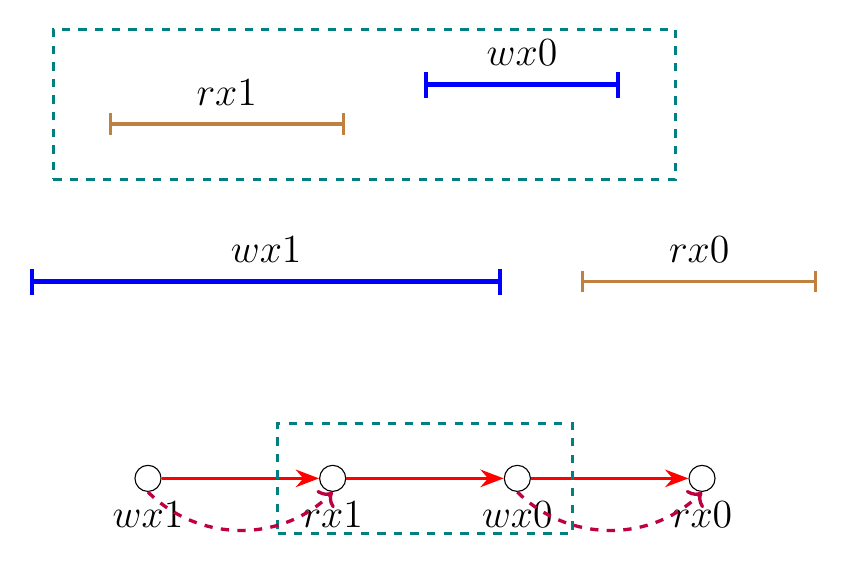
\begin{tikzpicture}[rf/.style = {->, bend right = 45, very thick, dashed, purple}]

  \itv{(0,0)}{(6,0)}{wx1}{ultra thick, blue};
  \itv{(7,0)}{(10,0)}{rx0}{very thick, brown};

  % \itv{(1,2)}{(3,2)}{wx0}{ultra thick, blue};
  \itv{(1,2)}{(4,2)}{rx1}{very thick, brown};
  \itv{(5,2.5)}{(7.5,2.5)}{wx0}{ultra thick, blue};

% atomicity schedule
\begin{scope}[font = \Large, start chain = atomicity, xshift = 1.5cm, yshift = -2.5cm, node distance = 2.0cm, every join/.style = {>=Stealth, very thick, ->, red}]
  \foreach \opi in {wx1, rx1, wx0, rx0}
    \node (\opi) [circle, draw, on chain, join, label = {[below] -90 : $\opi$}] {};
\end{scope}

% real-time order
\node () [draw, rectangle, inner sep = 20pt, teal, very thick, dashed, fit = (start rx1) (end wx0)] {};
\node () [draw, rectangle, inner sep = 15pt, teal, very thick, dashed, fit = (rx1) (wx0)] {};

% read-from relation
\draw[rf] (wx0.south) to (rx0.south);
\draw[rf] (wx1.south) to (rx1.south);

% show the meaning of "atomicity": linerization point
% \begin{scope}[atomicedge/.style = {>=Stealth, ->, dashed, draw, thick}]
%   \foreach \opi in {rx1, wx0, wx1, rx0}{
% 	\draw[atomicedge] (start \opi) to (\opi);
% 	\draw[atomicedge] (end \opi) to (\opi);
%   }
% \end{scope}
\end{tikzpicture}
\end{document}